\chapter{結論}
\newpage

\section{総括}
本研究では,上肢機能障害者支援を目指し,強化学習・深層学習をロボット制御に適用した自律型ロボットハンドの試作を行った.携帯可能な重量と人間の手と同等のサイズを目指して小型軽量化し,Cloudは使用せずEdgeのみで処理を実現した.今回開発したロボットハンドは指定した物体を識別し,接近し,把持し,使用者のもとへ運搬するタスクを達成できた.\fig{ロボットハンドまとめ}に今回試作したロボットハンドを並べて載せる.
\begin{figure}[H]
    \centering
    \begin{minipage}{0.65\hsize}
        \centering
        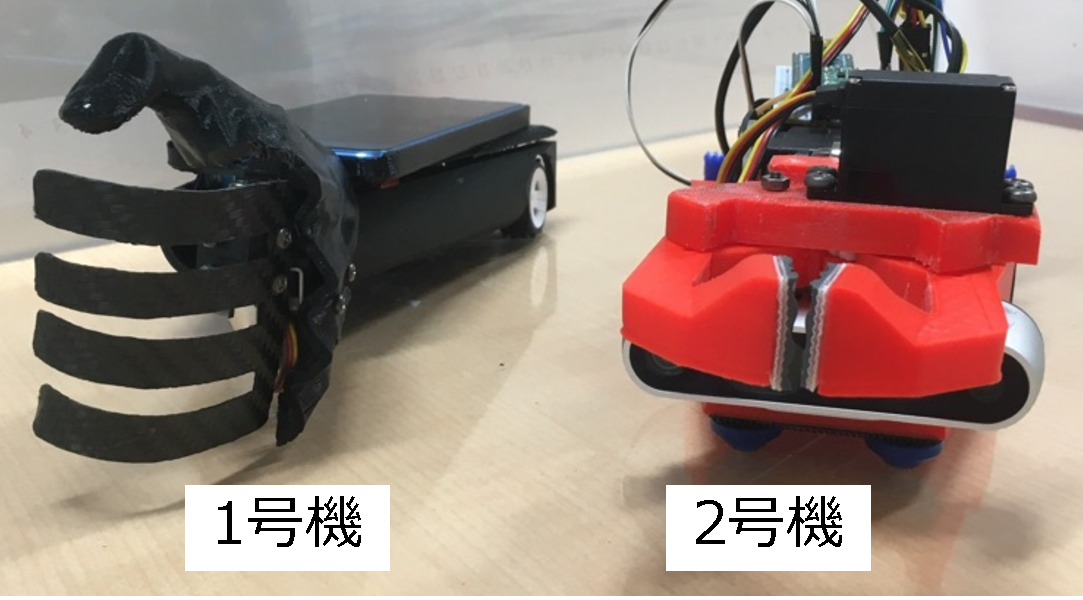
\includegraphics[width=\linewidth]{figure/chapter5/ロボットハンドまとめ前}
    \end{minipage}
    \hspace*{\fill}
    \begin{minipage}{0.32\hsize}
        \centering
        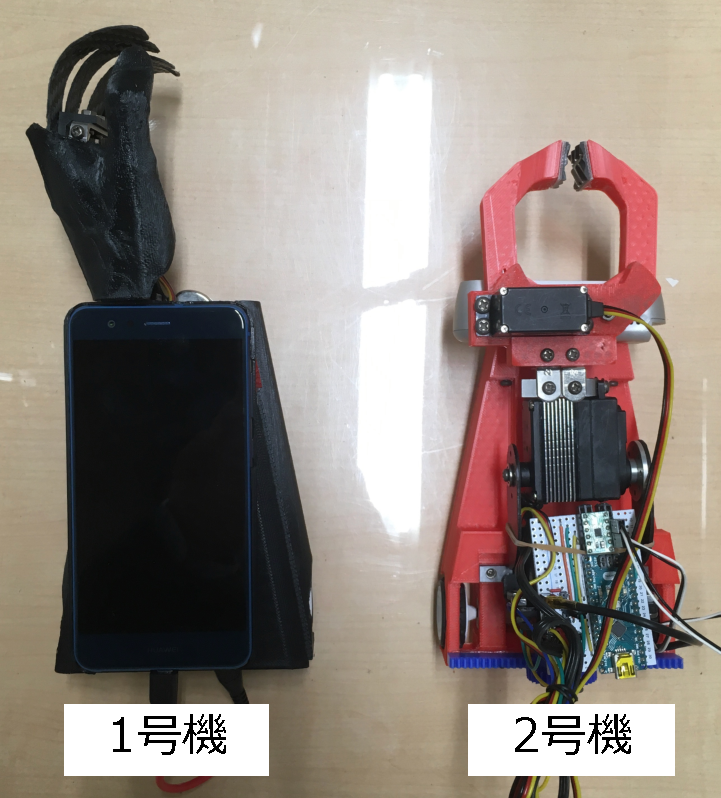
\includegraphics[width=\linewidth]{figure/chapter5/ロボットハンドまとめ上}
    \end{minipage}
    \caption{Apperarance of robot hands.}
    \label{fig:ロボットハンドまとめ}
\end{figure}
試作したロボットハンドそれぞれの特徴と課題について,以下にまとめる.

\subsection*{試作1号機}
1号機ではスマートフォンを搭載し,スマートフォンのカメラとCPUのみによる強化学習で,特定の色の物体への接近と把持に成功した.重量も一般的なパーソナルロボットよりも軽く(474 g),携帯する際使用者の負担にはならないと言える.リハビリテーション科に通う義手使用患者へヒアリングを実施した際も1号機は好評で,障害者支援への実用化が期待できる.

一方,計算リソースの制約から対象物の識別は不可能であり,事前に指定した物体の色のみの判断に留まった事が課題である.

\subsection*{試作2号機}
2号機では1号機と比べて,画像認識技術と深層学習により複数の物体がある中でも対象物を識別できるよう改善した.また,ロボットハンドの運動性能の自由度を増やし,物体を持ち上げて運搬することを可能にした.3種類の物体の識別を可能とし,ペットボトルの把持成功率は9割に達した.

一方,ロボットハンドの重量が軽いために,ロボット本体重量以上の重い物体を持ち上げることができなかった.これは本体の重心位置の最適化と本体重量増加で対応可能である.また,計算リソースの都合上GPUを搭載したデスクトップPCと有線で接続されているため,携帯性が低下した.これは次節で述べるように,より高性能のEdgeコンピュータを用いることで携帯性は大きく改善できる.


\section{今後の展望}\label{sec:今後の展望}
ロボットハンドの本体のデザイン,アクチュエータや計算リソースのハードウェア,アクチュエータの制御や画像処理を行うソフトウェアの3つの観点から,改善指針として以下にまとめる.

\subsection*{デザインの改善}
今回のロボットハンドでは,地面から直立している物体のみの把持は可能だが,紙や皿のような平たい物体や細長く自立困難な物体の把持は不可能であった.そのため,腕の関節と手首の関節を増やすことで地面に対して垂直にアプローチできるように改善することで,把持できる物体形状の幅が広がる.また,今回のグリッパは一般的な形状のものであったが,様々な物体を把持可能なJamming転移型グリッパ\cite{jamminggripper}など,グリッパ形状についても検討する必要がある.

\subsection*{ハードウェア(計算リソース)の改善}
2号機では識別能力を向上させるために,外部の計算リソースを使用していたためGPU搭載PCと有線で接続されていたことが実用化においては課題となる.そこで次世代機ではEdgeデバイス(例えばNVIDIA社のJetsonNanoボード)を使用することで,ロボットハンド自身でGPUを使用した推論が可能となる.さらにJetsonNanoを用いると直接アクチュエータの制御が可能となり,よりシンプルなロボット開発環境が実現できると考えられる.ただし,大きな消費電力が課題である.

\subsection*{ソフトウェアの改善}
接近タスクは比例制御で十分有効であることがわかったが,今回のロボットハンドでは一般的な2指対立タイプのグリッパを使用したこともあり,把持タスクはルールベースでは物体の形状に対称性が無いものは把持成功率が低かった.把持タスクにはVisionベースの教師あり学習を行い最適な把持点を掴むことで改善できる.さらに識別タスクに用いたMask R-CNNと合わせてモデルを構築できれば,End-to-Endに学習ができ精度改善や推論速度向上が期待できる.

また,今回タスクの指令はコマンドラインから行ったが,実際に使用するときは外部インターフェースが必要となる.インターフェースとしては音声コマンドやスマートフォンを使ったタッチパネル入力などが有用と考えられるが,使用者の障害に応じて検討する必要がある.
